\subsection{Lost Lepton background}
\label{sec:bkgLL}

The lost lepton background represents the total background contribution from all physics processes that contain two or more leptons from the hard scatter process, where only one of the leptons is reconstructed in the event.  The mis-reconstruction of the second lepton can contribute to the \MET in the event. Additionally, the presence of a second neutrino provides a large tails in the \MT and \MTtW distributions.  This type of background is thus the largest background in the signal region.  

The $\ttjets$ process, where $t\bar{t}\rightarrow\ell\ell$, is the dominant contribution to this background.  The single $t$ process, produced in association with a $W$ boson, where both the $W$ and the $t$-quark decay to leptons, accounts for the second-largest contribution.  Addtional contributions come from ${\ttbar}V$ and diBoson processes.  

The following describes a data-driven method to estimate this background, using a control region enriched in dilepton events.  


\subsubsection{Estimation method from data}
\label{sec:bkgLL:Data}

The lost lepton background is estimated from data in a control region that requires a second lepton, passing the \textit{veto} requirements, or the presence of an isolated track or tau. After the Monte Carlo has been corrected for differences in lepton and jet reconstruction efficiencies, with respect to the data, the ratio of events in the control region and signal regions, should be equivalent between the observed and simulated number of events.  This relationship is shown in eq.~\ref{eq:diLep_CR_ratios}.

\begin{equation}\label{eq:diLep_CR_ratios}
\frac{N^{Data,~Signal~Region}_{\ell\ell}}{N^{Data,~Control~Region}_{\ell\ell}} = 
\frac{M^{MC,~Signal~Region}_{\ell\ell}}{M^{MC,~Control~Region}_{\ell\ell}}
\end{equation}

For the purpose of shortness, we will denote the number of data events by $N$ or $N^{Data}$, while we denote the number of simulated events by $M$ or $M^{MC}$. Also signal regions are denoted by $SR$, while dileptonic control regions are denoted by $CR$.

A data-driven estimate for the number of events in the signal regions, can then be calculated by re-arranging eq.~\ref{eq:diLep_CR_ratios} to eq.~\ref{eq:diLep_SR_est_simple}

\begin{equation}\label{eq:diLep_SR_est_simple}
N^{SR}_{\ell\ell} = N^{CR}_{\ell\ell}\times
\frac{M^{SR}_{\ell\ell}}{M^{CR}_{\ell\ell}}
\end{equation}

To prevent signal contamination in the tails of \MET, and increase the statistics available for the measurement in those regions, events in this control region are only binned in low and high \MTtW, ($<$200 GeV, and $\ge$200 GeV respectively), and uses an inclusive selection of gen lepton decays.  {\color{red} What do you mean with an inclusive selection of gen lepton decays - I would drop it}. 
An additional transfer factor is thus needed in eq.~\ref{eq:diLep_SR_est_full} to account for the binning in the jet multiplicity (nJets) and \MET found in the signal regions.  The final form of the diLepton background estimate is then written as:

\begin{equation}\label{eq:diLep_SR_est_full}
N^{Data,~SR}_{\ell\ell} = N^{Data,~CR}_{incl~in~gen~lepton~decays}\times
\frac{M^{MC,~SR}_{\ell\ell}}{M^{MC,~CR}_{incl~in~gen~lepton~decays}}\times
\frac{M^{MC,~SR}_{\ell\ell,~nJet,~\MET~bin}}{M^{MC,~SR}_{\ell\ell}}
\end{equation}

The uncertainty on the signal region estimate is dominated by the statistical uncertainty on the number of events measured in data 
in the control region. %, i.e. the first term in \ref{eq:diLep_SR_est_full}.  
%An additional benefit of c
Combining the nJet and \MET bins is reducing this uncertainty.  

Two of the most important aspects of exploiting the equivalence of the ratio between signal and control regions, is the modelling of additional 
jets due to ISR/FSR radiation, and the modelling of the \MET spectrum.  
Each play important roles in accurately calculating the transfer factor for nJet and \MET bins, but the additional jet modelling also comes 
into play in the differences between the signal and control regions as well. 
Therefore, a dedicated, low \MET, dilepton control region will be 
used to measure the jet multiplicity for $t\bar{t}$, and correct the simulation accordingly.      

\subsubsection{Addtional Control Region to Evaluate $t\bar{t}$ modelling}
\label{sec:bkgLL:emu_CR}

An additional control region is formed to study the simulation of the \ttjets background.  This region is used to derive an additional scale factor for the signal and control regions.  Approximately half the lost lepton background is composed of hadronic tau decays.  The other half, decays with a lost $e$ or $\mu$, need an additional ISR/FSR jet relative to the hadronic tau component of the lost lepton background, as shown in equation \ref{eq:emu_CR:xsecs}, in order to pass the jet selection requirements. 

%\begin{equation}
\begin{align} \label{eq:emu_CR:xsecs}
N^{SR}_{\ell\tau} &= (\sigma^{+1j}_{2\ell})\ast\epsilon_{reco~\ell}\ast(1-\epsilon_{reco~\tau})\ast\epsilon_{selection}\ast\epsilon_{reco~\tau~as~jet} \\
N^{SR}_{\ell\ell} &= (\sigma^{+2j}_{2\ell})\ast\epsilon_{reco~\ell}\ast(1-\epsilon_{reco~\ell})\ast\epsilon_{selection}
\end{align}
%\end{equation}

{\color{red} What is $\epsilon_{reco~\tau~as~jet}$. Basically every tau is a jet unless it is outside jet acceptance}.

Here, $\epsilon_{selection}$ is the total selection efficiency but the part coming from the leptons, which is encoded in the terms with $\epsilon_{reco~X}$.
For our signal regions, $\ttbar\to2\ell$ has - on tree level, just two jets in the event, while $\ttbar\to1\ell$ or signal has four jets (two jets from the hadronic W boson decay).

Events due to $\ttbar\to2\ell$, where the lost lepton is a hadronic tau, we need to find one additional ISR/FSR jet to pass our event selection, as the tau lepton itself is already identified as jet ($\rightarrow \sigma^{+1j}_{2\ell}$).
If however, the lost lepton is due to a missed e or $\mu$, we need at least two addition ISR/FSR jets ($\rightarrow \sigma^{+2j}_{2\ell}$).

When forming the ratio for the diLepton control region to the signal region (second factor in eq.~\ref{eq:diLep_SR_est_full}), 
the lepton reconstruction efficiencies will effectively cancel %due to their similarities in the denominator and numerator, 
and the only difference will be in the modelling of the cross section for additional ISR/FSR jets.  The scale factors are calculated as the 
ratio of ratios between data and Monte Carlo for jet bins of $=3/=2$ and $\ge4/=2$ jets.

The selection for this region is motivated to achieve a high-purity $t\bar{t}$ sample of events in data:

\begin{itemize}
  \item Pass an $e,\mu$ diLepton trigger
  %\begin{itemize}
   % \item HLT\_Mu17\_TrkIsoVVL\_Ele12\_CaloIdL\_TrackIdL\_IsoVL\_v*
   % \item HLT\_Mu23\_TrkIsoVVL\_Ele12\_CaloIdL\_TrackIdL\_IsoVL\_v*
  %\end{itemize}
  \item exactly 2 leptons
  \begin{itemize}
    \item e and $\mu$ flavour selection
    \item $\pt>30(15)\GeV$ leading (trailing) leptons 
    \item $|\eta|<2.1$
    \item POG ID medium (tight) for $e (\mu)$
    \item relative mini isolation $<0.1$
    \item oppositely charged
  \end{itemize}
  \item diLepton mass, $m_{\ell\ell}>20\GeV$
  \item nJets$\ge2$
  \item nBTags$\ge0$
\end{itemize}

We call this control region $CR_{e\mu}$. {color{red} Are you ok with that?}
The yields for this region are given in the following table \ref{tab:emu_CR:yields}.  Uncertainties are statistical only.  

\begin{table}[htb]
\begin{center}
\small
\caption{\label{tab:emu_CR:yields} Yield table for 2.11$fb^{1}$ of data for the $e,\mu$ control region, in bins of nTags}
\begin{tabular}{|l|c|c|c|c|} \hline
 & $CR_{e\mu},~\ge0~b-tags$ & $CR_{e\mu},~\ge1~b-tags$ & $CR_{e\mu},~\ge2~b-tags$ \\ \hline
Rare & 155.35 $\pm$ 1.28  & 30.33 $\pm$ 0.47  & 7.92 $\pm$ 0.21 \\ \hline
$W$+Jets, madgraph & 17.14 $\pm$ 1.71  & 2.97 $\pm$ 0.73  & 0.05 $\pm$ 0.02 \\ \hline
DY+Jets, amcnlo & 161.42 $\pm$ 17.86  & 22.07 $\pm$ 5.68  & 4.02 $\pm$ 2.34 \\ \hline
Single $t$, powheg & 403.17 $\pm$ 5.44  & 273.93 $\pm$ 4.38  & 64.94 $\pm$ 2.06 \\ \hline
$t\bar{t}$, 1l, powheg ext & 92.45 $\pm$ 1.28  & 52.74 $\pm$ 0.94  & 7.59 $\pm$ 0.35 \\ \hline
$t\bar{t}$, 2l, powheg ext & 7921.71 $\pm$ 11.85  & 6137.61 $\pm$ 10.21  & 2193.36 $\pm$ 5.85 \\ \hline
Total Background & 8751.32 $\pm$ 22.25  & 6519.69 $\pm$ 12.54  & 2277.90 $\pm$ 6.65 \\ \hline
Data & 8618  & 6333  & 2129 \\ \hline
Data/simulation & 0.98 $\pm$ 0.00  & 0.97 $\pm$ 0.00  & 0.93 $\pm$ 0.00 \\ \hline
\end{tabular}
\end{center}
\end{table}

The region of highest $t\bar{t}{\rightarrow}2\ell$ purity is the nBTags$\ge$2 category.  Therefore, this will be the region used to extract the correction factors for the $==3$ and $\ge4$ jet bins.  These factors will be applied to $t\bar{t}{\rightarrow}2\ell$ events in both the signal region, and nominal diLepton control region used to derive the signal estimate.   

The distributions of number of jets in each event, for increasing \MET cuts are shown in figure \ref{fig:bkgLostLepton:nJets}

\begin{figure}[ht]
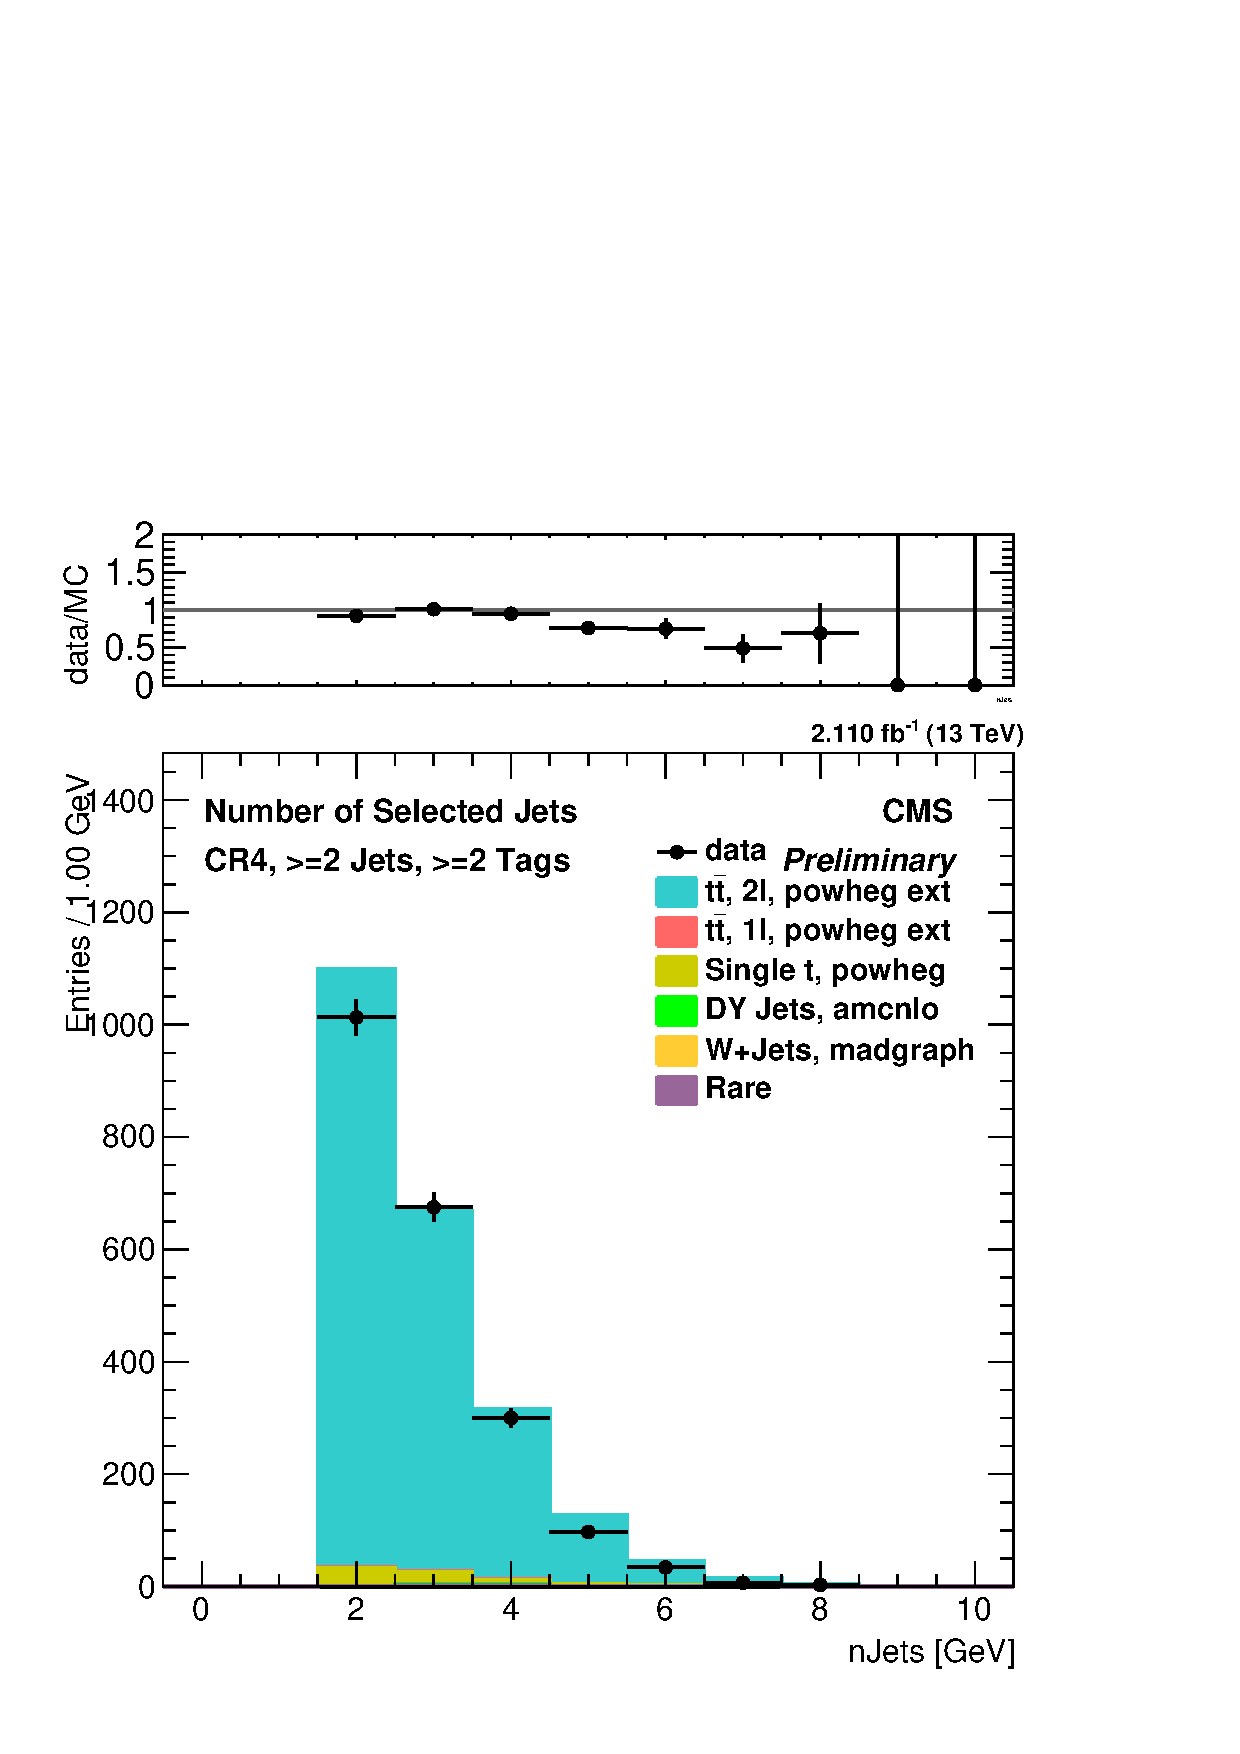
\includegraphics[width=0.32\textwidth]{Figures/bkgLostLepton/data_MC_plot__byProductionMode__nJets__elmu__ge2j_ge2t_gt0met__linScale.pdf}
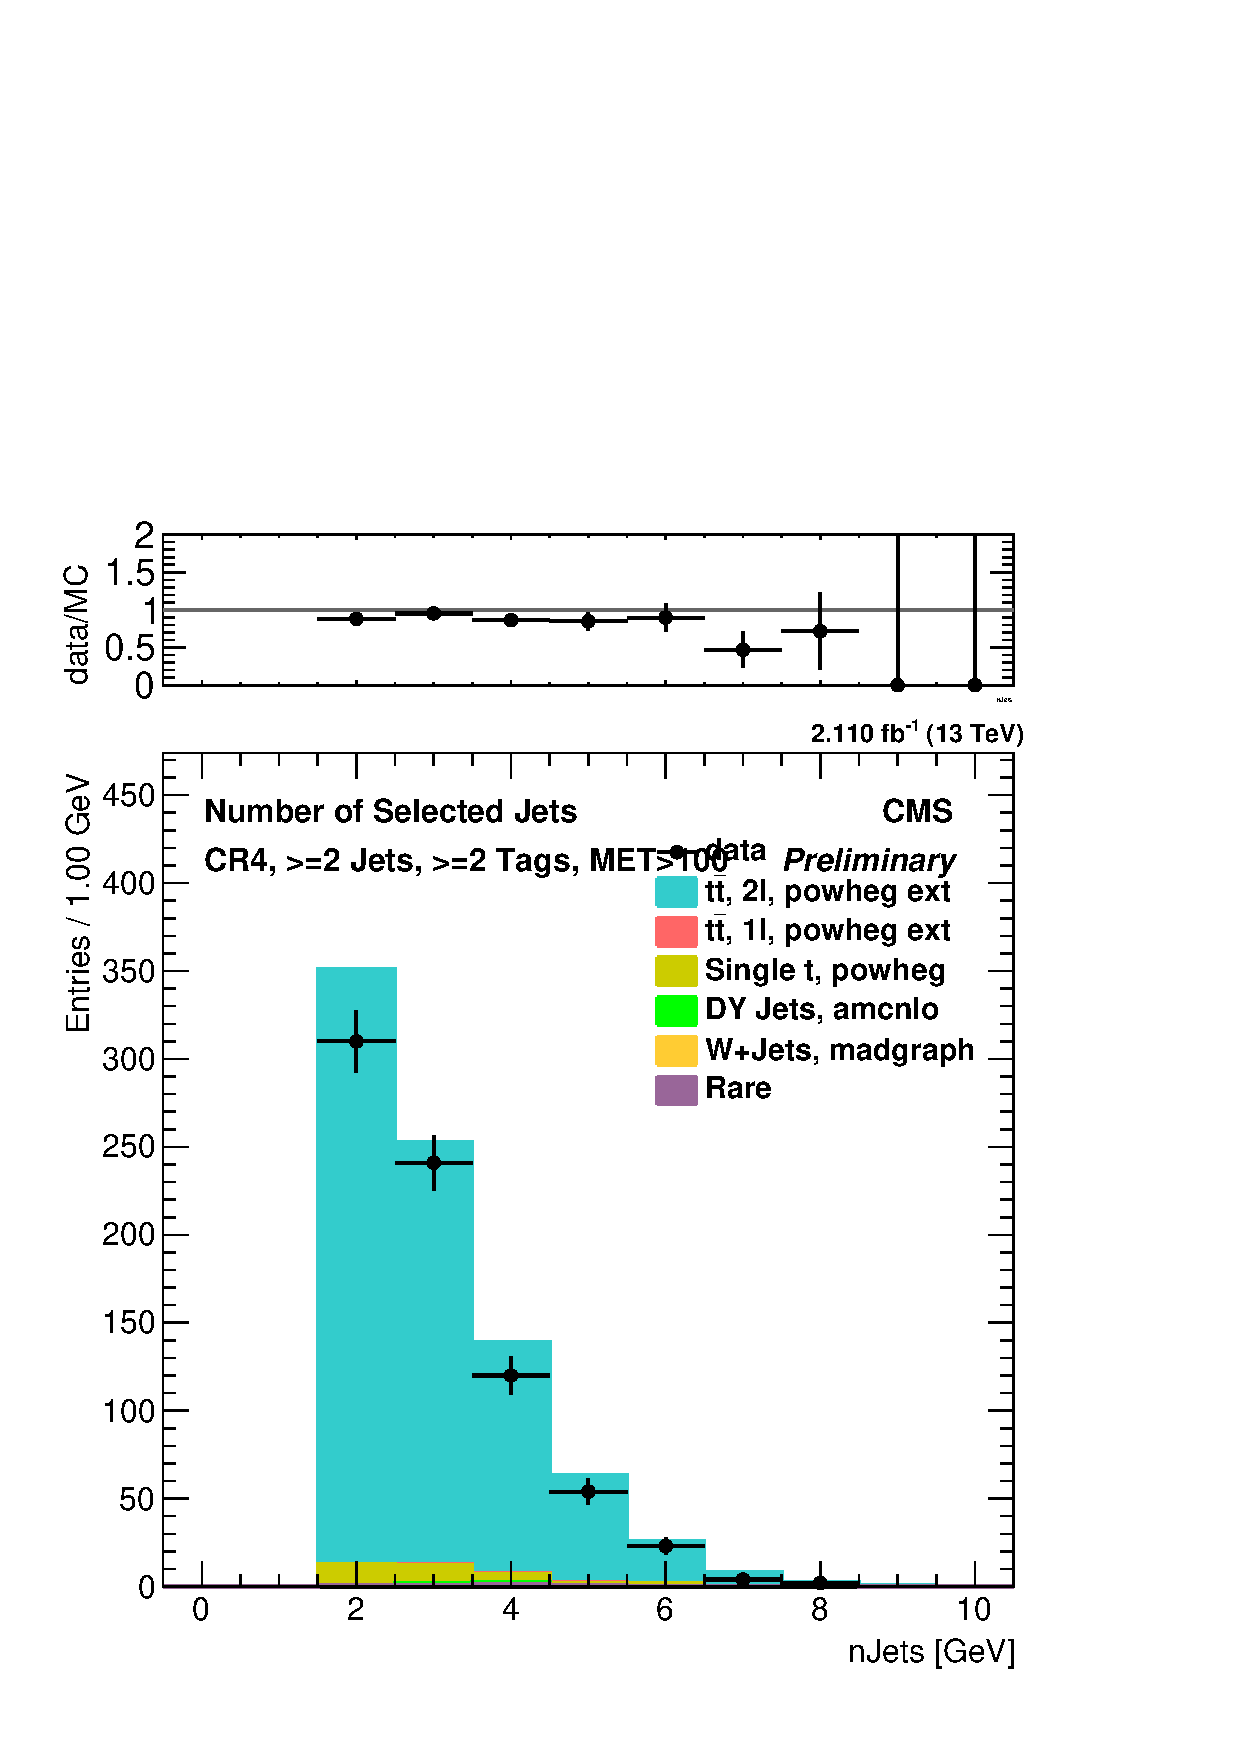
\includegraphics[width=0.32\textwidth]{Figures/bkgLostLepton/data_MC_plot__byProductionMode__nJets__elmu__ge2j_ge2t_gt100met__linScale.pdf}
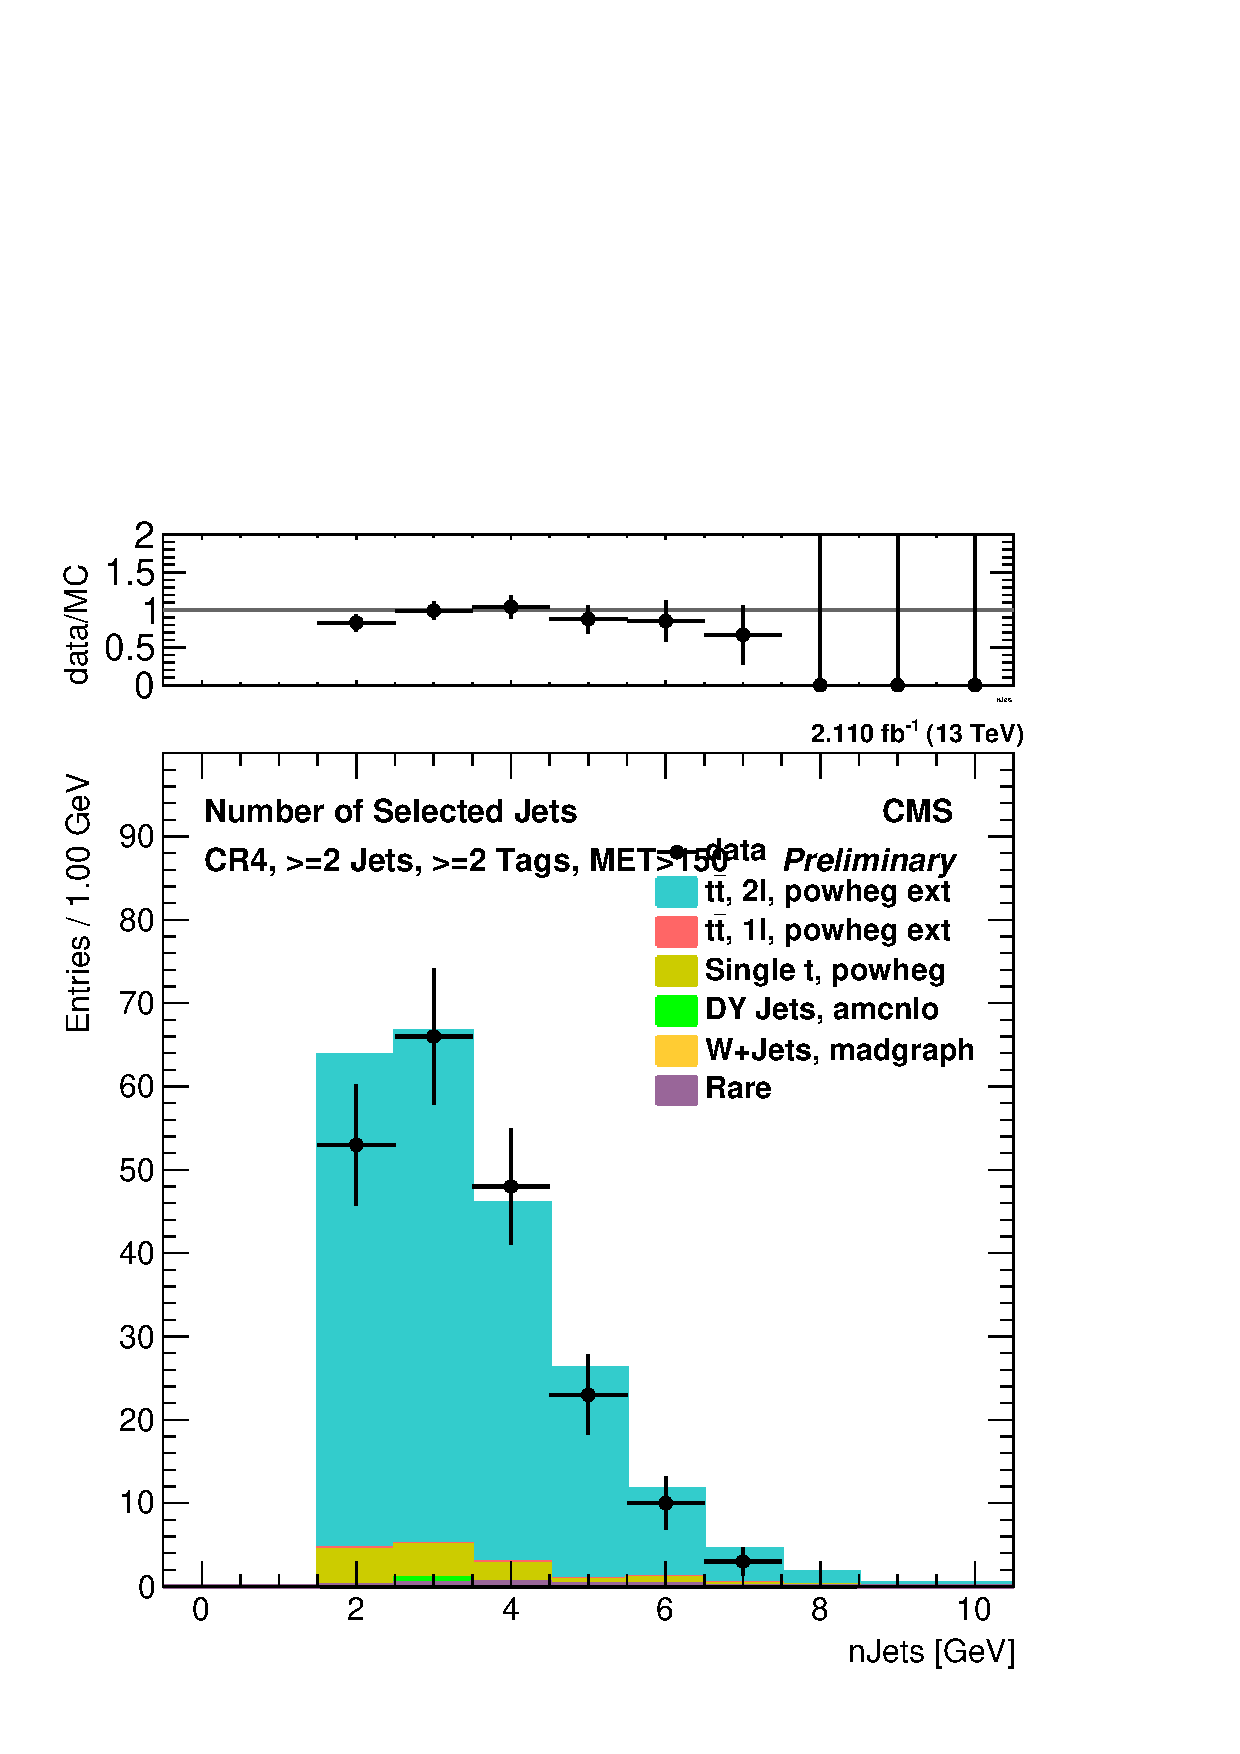
\includegraphics[width=0.32\textwidth]{Figures/bkgLostLepton/data_MC_plot__byProductionMode__nJets__elmu__ge2j_ge2t_gt150met__linScale.pdf}
\caption{\label{fig:bkgLostLepton:nJets} Distribution of number of jets for \MET$>$50 GeV (left), \MET$>$100 GeV (center), \MET$>$150 GeV}
\end{figure}

The scale factor derived from the nJets distribution in this region is given in table \ref{tab:emu_CR:SF}.  Within the statistical uncertainties quoted, the factors K3, and K4 are flat with increasing \MET. Thus, the most inclusive \MET bin will be used for the calculation, giving:

\begin{itemize}
  \item K3 = 1.10$\pm$0.06
  \item K4 = 0.94$\pm$0.06
\end{itemize}

\begin{table}[htb]
\begin{center}
\small
\caption{\label{tab:emu_CR:SF} Table of Scale Factors as a function \MET}
\begin{tabular}{|l|c|c|} \hline
Category & $nJets=3~(K_{3})$ & $nJets>=4~(K_{4})$ \\ \hline
$CR_{e\mu}, \ge2~b-tags, \MET\ge0\GeV$  & 1.10 $\pm$ 0.06 & 0.94 $\pm$ 0.06\\ \hline
$CR_{e\mu}, \ge2~b-tags, \MET>100\GeV$  & 1.08 $\pm$ 0.10 & 0.95 $\pm$ 0.09\\ \hline
$CR_{e\mu}, \ge2~b-tags, \MET>150\GeV$  & 1.21 $\pm$ 0.25 & 1.12 $\pm$ 0.22\\ \hline
$CR_{e\mu}, \ge2~b-tags, \MET>200\GeV$  & 1.42 $\pm$ 0.85 & 1.65 $\pm$ 0.89\\ \hline
\end{tabular}
\end{center}
\end{table}

%\subsubsection{High \MET diLepton Control Region used for Signal Region estimates}
\subsubsection{DiLepton Control Region used for Signal Region estimates}
\label{sec:bkgLL:highMET_CR}
 
As mentioned before, we estimate the lost lepton background by extrapolation 
in lepton veto, \MET, and Njets from appropriately chosen control regions.  
In the present section we document the control region definitions, control region yields, extrapolation
factors after all corrections, and the resulting estimates for lost lepton background yields in all signal regions.

We define two control regions (CR), one for MT2W$<$200 GeV, and one for MT2W$\ge$200 GeV.
For both region we require \MET $\ge$ 250 GeV, $\ge $ 3 jets, and one of the following lepton selections:

\begin{itemize}
    \item Require =2 leptons passing analysis selections, and $p_{T} >$ 20 GeV.
    \item Require =1 lepton passing analysis selection ($p_{T}>$ 20 GeV), and ==1 lepton passing veto selection ($p_{T}>$ 10 GeV).
    \item Require =1 lepton passing analysis selection, ==0 leptons passing veto selection, 
          and either an isolated track ($p_{T}>$ 10 GeV), or hardronic tau ($p_{T}>$ 20 GeV visible transverse momentum), 
          identified by the same requirements as the isolated track and tau vetoes.  
\end{itemize}

%This implies that there are exactly two control regions used to estimate the lost lepton backgrounds for all the signal regions.
The yields for both are given in the top two rows of Table \ref{tab:diLeptonType_Data_MC}.

In order to test the \MET modelling, we divide the some of those control region %\MET$\ge$ 250 GeV range 
into three subranges of roughly equal expected yield, and check
for any dependence of the Data/simulation yield ratio across \MET. We see no trend. %in this cross check. 
This is also documented in Table~\ref{tab:diLeptonType_Data_MC}.
Figure \ref{fig:cr_data_mc} provides a visual representation of the that table.  The uncertainties are statistical only. 
Additionally, the \MET and \MTtW distributions, are shown in figure \ref{fig:cr_data_mc:met_mt2w}.

\begin{table}[htb]
\begin{center}
\small
\caption{\label{tab:diLeptonType_Data_MC} Total event yields for each type of diLepton classification for data and MC, for 2.11$fb^{-1}$ }
\begin{tabular}{|l|c|c|c|} \hline
 Category & Data & MC & Data/MC \\ \hline
 $CR,~\ge3~jets,~\MET\ge250\GeV,~\MTtW<200\GeV$ & 66 $\pm$ 8.12 & 67.00 $\pm$ 1.14 & 0.99 $\pm$ 0.12 \\ \hline
 $CR,~\ge3~jets,~\MET\ge250\GeV,~\MTtW\ge200\GeV$ & 18 $\pm$ 4.24 & 25.55 $\pm$ 0.89 & 0.70 $\pm$ 0.17 \\ \hline\hline
 $CR,~\ge3~jets,~250<\MET<275\GeV$ & 27 $\pm$ 5.20 & 30.83 $\pm$ 0.80 & 0.88 $\pm$ 0.17 \\ \hline
 $CR,~\ge3~jets,~275<\MET<325\GeV$ & 31 $\pm$ 5.57 & 33.04 $\pm$ 0.86 & 0.94 $\pm$ 0.17 \\ \hline
 $CR,~\ge3~jets,~\MET>325\GeV$ & 26 $\pm$ 5.10 & 28.69 $\pm$ 0.85 & 0.91 $\pm$ 0.18 \\ \hline
\end{tabular}
\end{center}
\end{table}

\begin{figure}[ht]
\centering
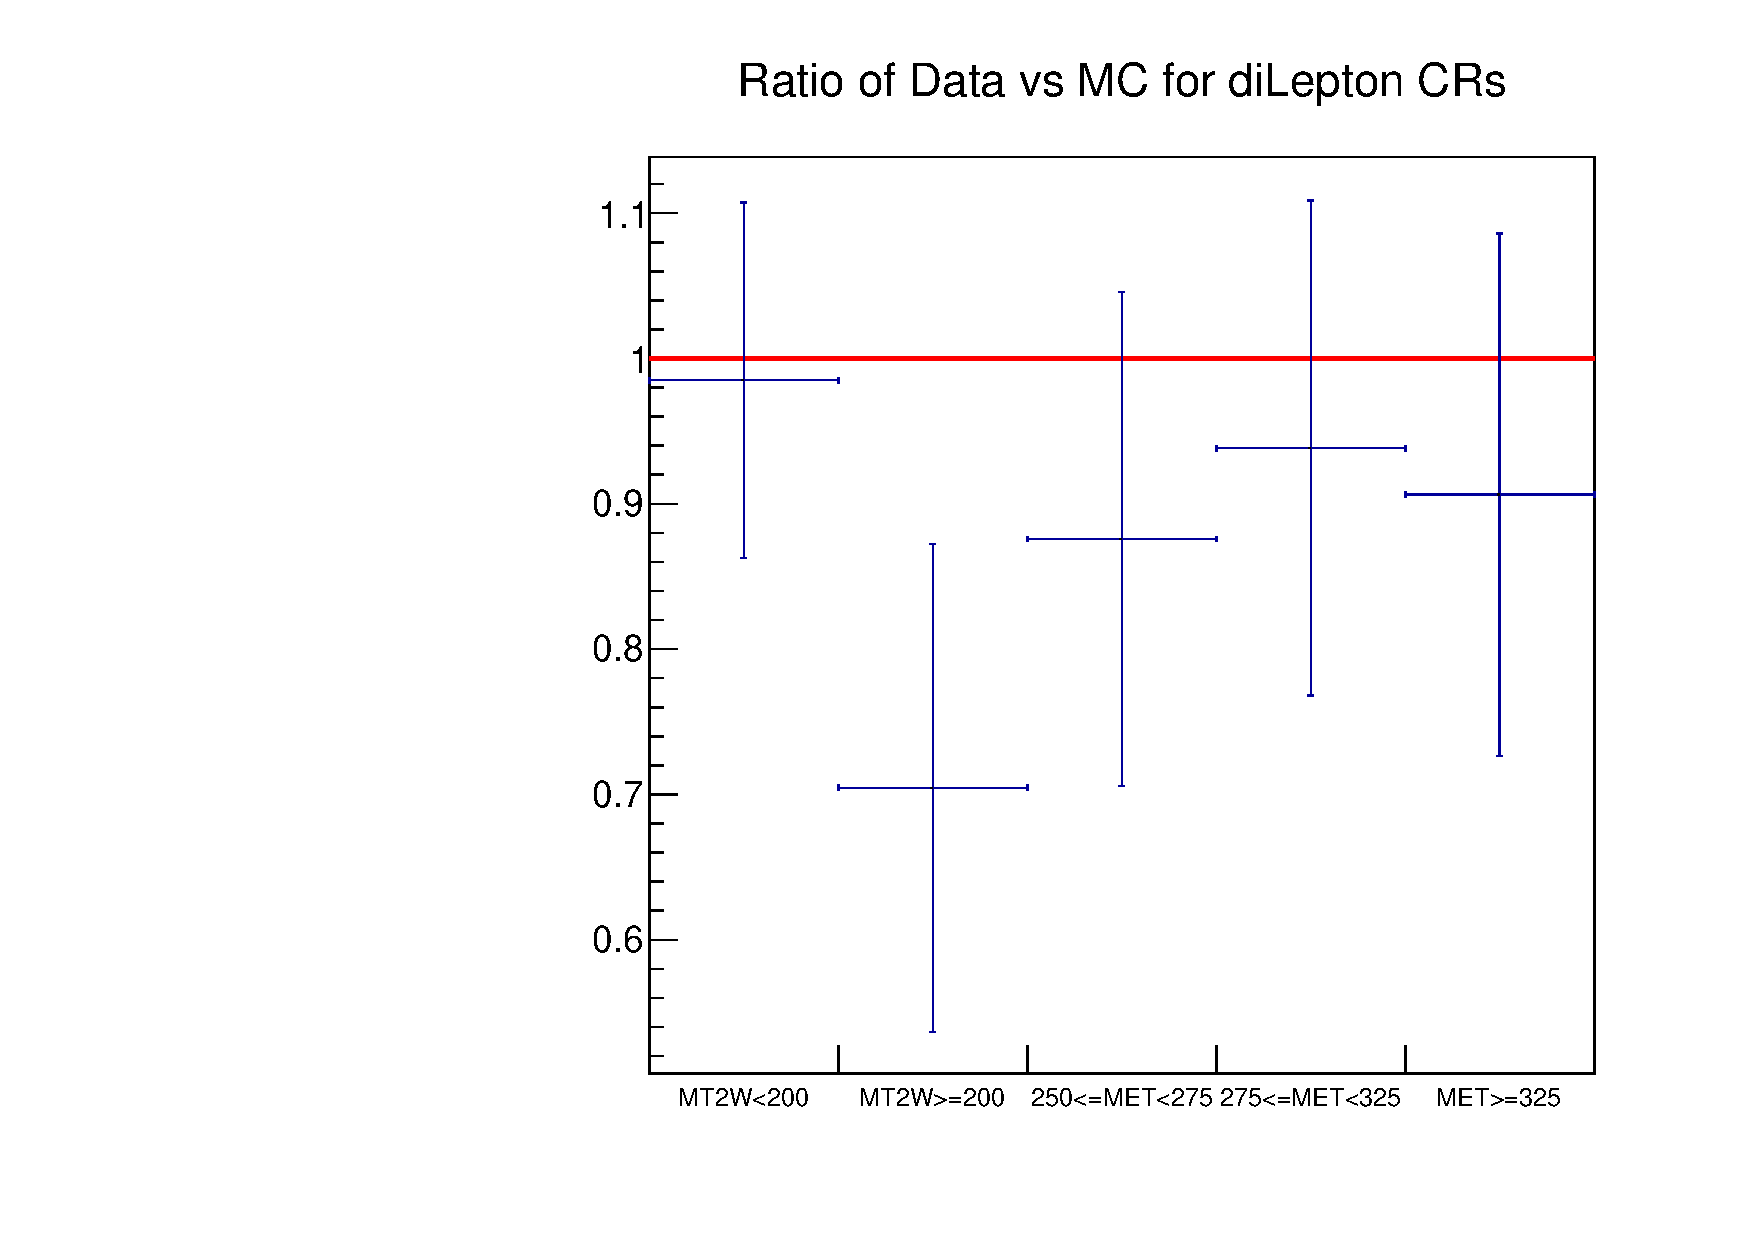
\includegraphics[width=0.70\textwidth]{Figures/bkgLostLepton/data_vs_mc__diLep_CR4_5_6__ge3j__ge250met__ratioOfCRs.pdf}
\caption{\label{fig:cr_data_mc} Data vs MC comparisons of the 5 bins used to evaluate the control region}
\end{figure}


\begin{figure}[ht]
\centering
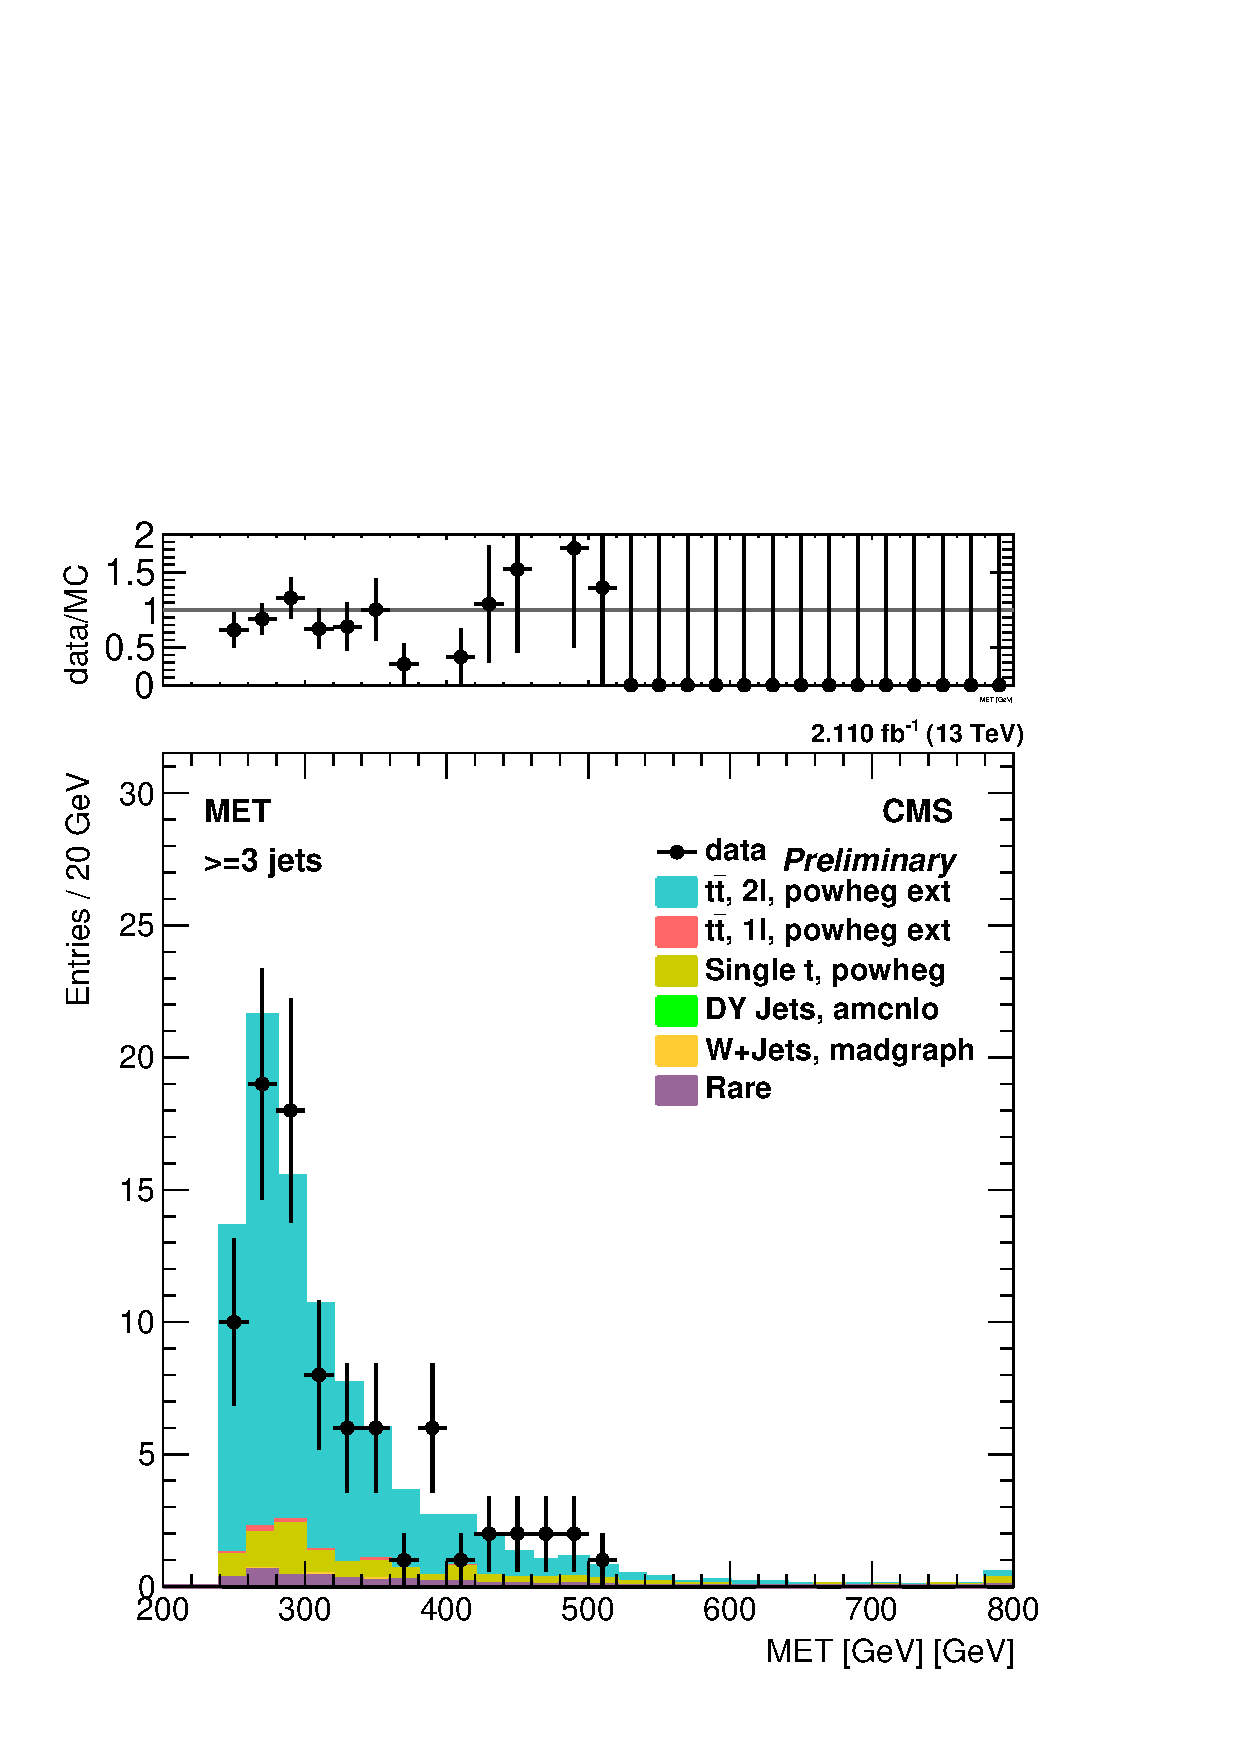
\includegraphics[width=0.45\textwidth]{Figures/bkgLostLepton/data_MC_plot__byProductionMode__met__ge3j_ge250met__linScale.pdf}
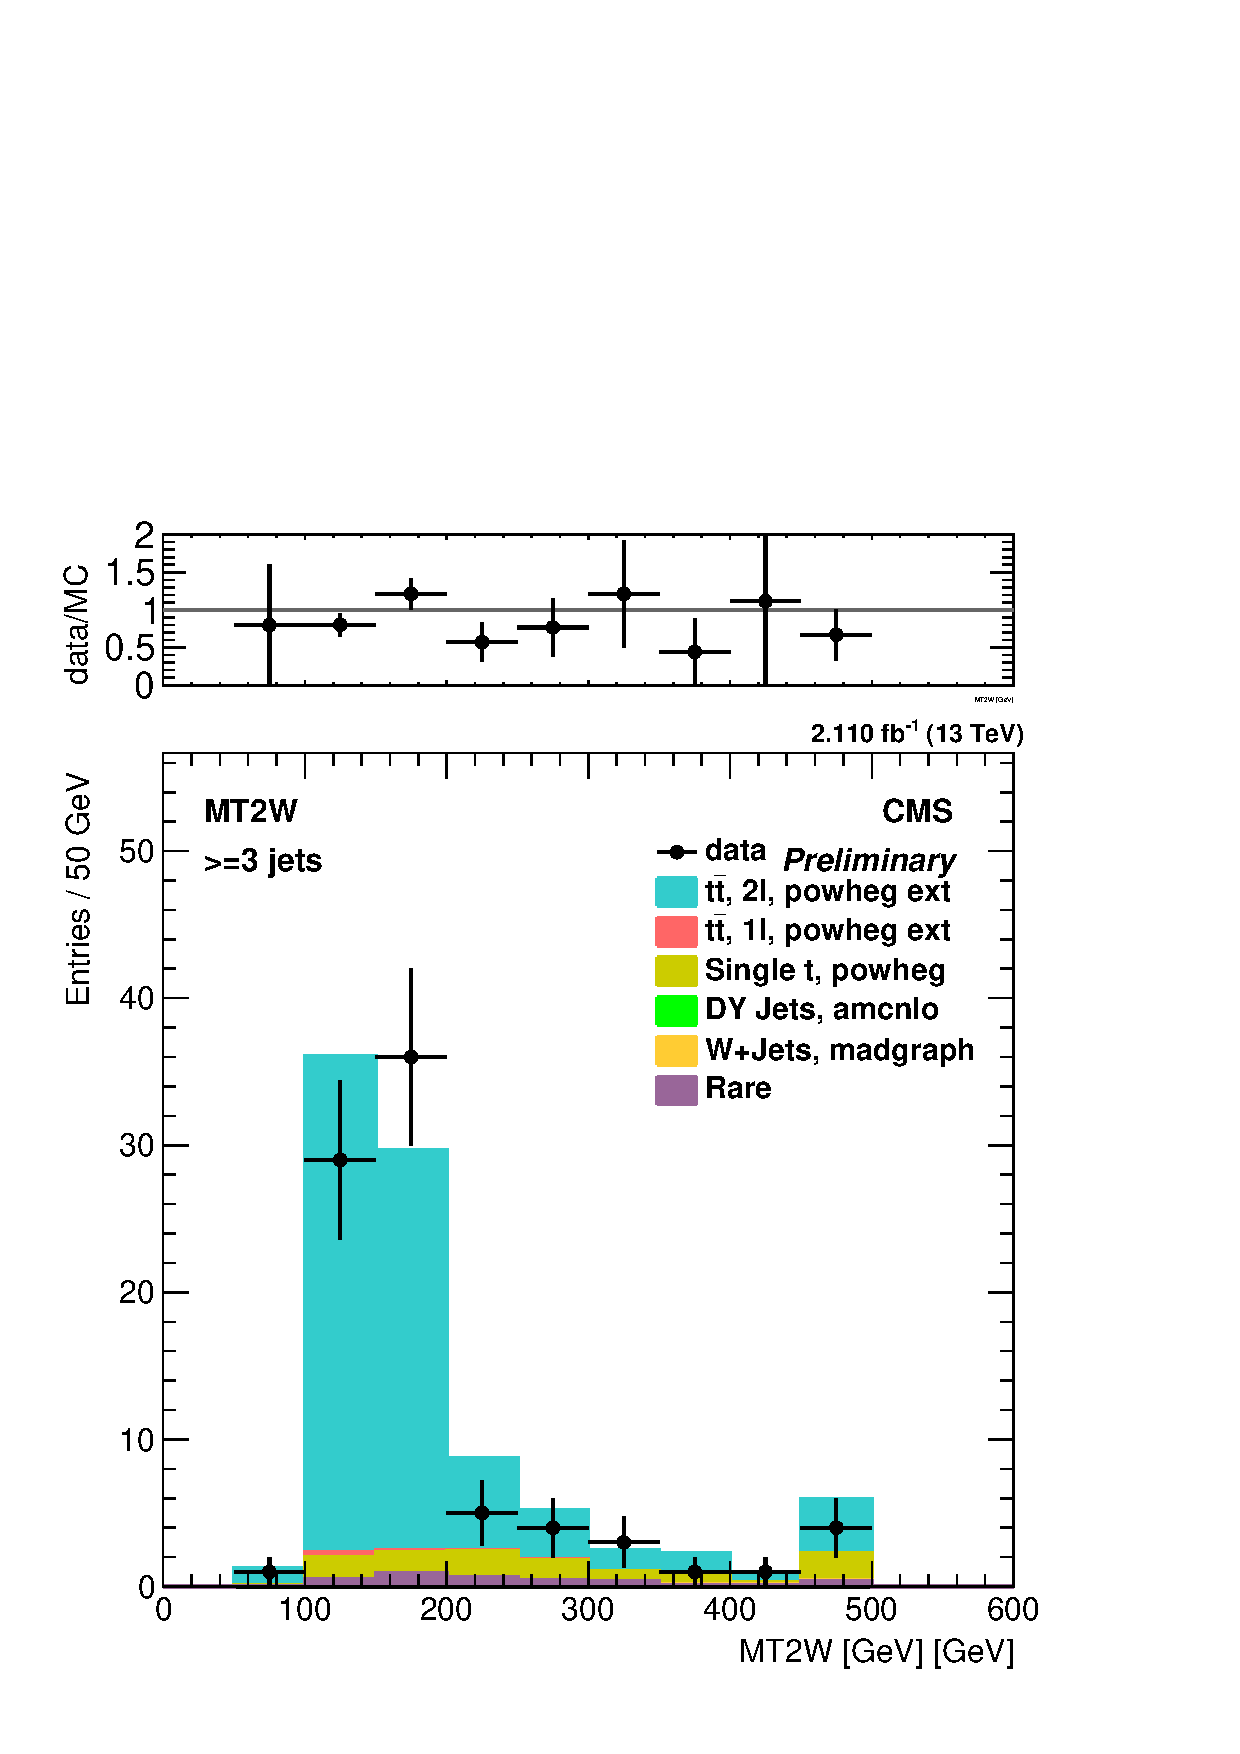
\includegraphics[width=0.45\textwidth]{Figures/bkgLostLepton/data_MC_plot__byProductionMode__mt2w__ge3j_ge250met__linScale.pdf}
\caption{\label{fig:cr_data_mc:met_mt2w} Distribution of \MET and MT2W in the diLepton CR}
\end{figure}


The resulting background yield predictions for each signal region are described in table \ref{tab:sr_estimate_lostLep}.  
The uncertainties here include the full systematic uncertainties from lepton, jet, and bTagging scale factors, 
as well as acceptance uncertainties from $Q^{2}$ and $\alpha_{S}$ variations, that are described in more detail in the 
following section.

%\subsubsection{High \MET diLepton Control Region used for Signal Region estimates, Systematic Uncertainties}
\subsubsection{Systematic Uncertainties for the lost lepton background estimation}
\label{sec:bkgLL:highMET_CR:systematics}

The full list of systematics used to evaluate the uncertainty on the diLepton background estimate is shown in table \ref{tab:ll_estimate_sysUnc_summary}.  

\begin{table}[htb]
\begin{center}
\small
\caption{\label{tab:ll_estimate_sysUnc_summary} Table of uncertainties for the diLepton background estimate, range for smallest-largest variation in each signal region. }
\scalebox{0.9}{
\begin{tabular}{|l|c|c|c|c|} \hline
Systematic & $N_{Incl}^{CR}~(\%)$ & $M_{2\ell}^{SR}/M_{Incl}^{CR}~(\%)$ & $M_{MET,nJet~bin}^{SR}/M_{2\ell}^{SR}~(\%)$ & $N_{2\ell,estimate}^{SR}~(\%)$ \\ \hline \hline
%Data Stats & $12.3~-~23.6~\%$ & $0.0~-~0.0~\%$ & $0.0~-~0.0~\%$ & $12.3~-~23.6~\%$ \\ \hline
%MC Stats & $0.0~-~0.0~\%$ & $1.7~-~3.5~\%$ & $2.1~-~11.6~\%$ & $2.7~-~12.1~\%$ \\ \hline
%$Luminosity$ & $0.0~-~0.0~\%$ & $0.0~-~0.0~\%$ & $0.0~-~0.0~\%$ & $0.0~-~0.0~\%$ \\ \hline
%$bTag~Efficiency,~Heavy~Flavour$ & $0.0~-~0.0~\%$ & $0.3~-~0.3~\%$ & $0.0~-~1.3~\%$ & $0.2~-~1.5~\%$ \\ \hline
%$bTag~Efficiency,~Light~Flavour$ & $0.0~-~0.0~\%$ & $1.4~-~2.1~\%$ & $0.0~-~0.9~\%$ & $0.9~-~2.3~\%$ \\ \hline
%$lepton~SF$ & $0.0~-~0.0~\%$ & $3.9~-~4.3~\%$ & $0.1~-~3.7~\%$ & $3.2~-~8.0~\%$ \\ \hline
%$top~p_{T}~SF$ & $0.0~-~0.0~\%$ & $0.3~-~2.8~\%$ & $0.2~-~13.5~\%$ & $0.2~-~13.7~\%$ \\ \hline
%$nJets~SF,~K3,~K4$ & $0.0~-~0.0~\%$ & $0.1~-~0.6~\%$ & $0.1~-~1.3~\%$ & $0.2~-~1.1~\%$ \\ \hline
%$PDF$ & $0.0~-~0.0~\%$ & $0.2~-~0.6~\%$ & $0.1~-~0.7~\%$ & $0.0~-~1.2~\%$ \\ \hline
%$\alpha_{S}$ & $0.0~-~0.0~\%$ & $0.1~-~0.4~\%$ & $0.0~-~0.5~\%$ & $0.0~-~0.6~\%$ \\ \hline
%$Q^{2}$ & $0.0~-~0.0~\%$ & $0.3~-~4.1~\%$ & $0.4~-~8.4~\%$ & $0.4~-~12.9~\%$ \\ \hline
%JES & $0.0~-~0.0~\%$ & $0.4~-~4.1~\%$ & $1.1~-~11.5~\%$ & $1.5~-~8.3~\%$ \\ \hline \hline
%Total & $12.3~-~23.6~\%$ & $5.6~-~8.2~\%$ & $3.6~-~20.1~\%$ & $14.6~-~34.0~\%$ \\ \hline
Data Statistics & $12.3~-~23.6~\%$ & --- & --- & $12.3~-~23.6~\%$ \\ \hline
Simulation Statisticss & --- & $1.7~-~3.5~\%$ & $2.1~-~11.6~\%$ & $2.7~-~12.1~\%$ \\ \hline
%Luminosity & --- & --- & --- & --- \\ \hline
bTag~Efficiency,~Heavy~Flavour & --- & $0.3~-~0.3~\%$ & $0.0~-~1.3~\%$ & $0.2~-~1.5~\%$ \\ \hline
bTag~Efficiency,~Light~Flavour & --- & $1.4~-~2.1~\%$ & $0.0~-~0.9~\%$ & $0.9~-~2.3~\%$ \\ \hline
lepton~SF & --- & $3.9~-~4.3~\%$ & $0.1~-~3.7~\%$ & $3.2~-~8.0~\%$ \\ \hline
top~\pt~SF & --- & $0.3~-~2.8~\%$ & $0.2~-~13.5~\%$ & $0.2~-~13.7~\%$ \\ \hline
nJets~SF,~K3,~K4 & --- & $0.1~-~0.6~\%$ & $0.1~-~1.3~\%$ & $0.2~-~1.1~\%$ \\ \hline
PDF & --- & $0.2~-~0.6~\%$ & $0.1~-~0.7~\%$ & $0.0~-~1.2~\%$ \\ \hline
$\alpha_{S}$ & --- & $0.1~-~0.4~\%$ & $0.0~-~0.5~\%$ & $0.0~-~0.6~\%$ \\ \hline
$Q^{2}$ & --- & $0.3~-~4.1~\%$ & $0.4~-~8.4~\%$ & $0.4~-~12.9~\%$ \\ \hline
JES & --- & $0.4~-~4.1~\%$ & $1.1~-~11.5~\%$ & $1.5~-~8.3~\%$ \\ \hline \hline
Total & $12.3~-~23.6~\%$ & $5.6~-~8.2~\%$ & $3.6~-~20.1~\%$ & $14.6~-~34.0~\%$ \\ \hline
\end{tabular}
}
\end{center}
\end{table}



The uncertainties are described as follows:
\begin{itemize}
  \item Data and MC statisitics - the largest uncertainty is due to the statistical error on the observed control region yields in data.
  \item nJets K3, K4 - impact of the statistical errors on the nJets scale factors applied to $\ttbar\to2\ell$, as described in the previous section. 
  \item bTagging Heavy/Light Flavour, SF - the variation of the heavy/light flavour component of the bTagging reweighting, as provided by the BTV POG.
%  \item bTagging Light Flavour, SF - the variation of the light flavour component of the bTagging reweightingm as provided by the BTV POG.
  \item lepton SF - the varation of the lepton scale factors, as provided by the SUSY group.  Scale factors for both ID and isolation are applied.
  \item top pT  - although the reweighting is not applied as a scale factor, an additional uncertainty is taken to account for the difference in yields if the reweighting is applied, as recommended by the top PAG. 
  \item PDF - the method used is to take the average of 100 different PDF variations, and use the standard deviation of this average to vary the acceptance on the MC
  \item $\alpha_{S}$ - this method varies the QCD scale of the event to change the acceptance. 
  \item $Q^{2}$ - the largest two variations in renormalization and factorization scale are taken as an envelope.  
  \item JES - the jet energy scale is varied, to account for diffences in jet acceptance.  
\end{itemize}

The latter uncertainties only consider the change in acceptance, but not in cross-section as we obtain the cross section from the data yields.

Even, if we write out the estimation formula as in eq.~\ref{eq:diLep_SR_est_full}, we do not double count uncertainties due to cancelling terms in that equation.

{\bf fkw comment: We are still missing the impact of possible \MET resolution difference between data and MC on
     possible bin migration in \MET,and corresponding impact on the \MET extrapolation. I.e. this is HJ's photon sample
     technique applied to the lost lepton bkg estimate. I thought we decided to do this at our f2f meeting at fnal.}
{\color{red} HJ: Do we need this here. We thought the main contribution of the \MET shape is due to real \MET. Possible mismodelling should (partially) taken care of JES. Anyway, I think John is implementing it, and as soon as it is in, I'll add a short paragraph, with forward-reference to the WJets section.}

\subsection{Results of the lost lepton background estimation}
\label{sec:bkgLL:highMET_CR:results}

\begin{table}[htb]
\begin{center}
\small
\caption{\label{tab:sr_estimate_lostLep} Total event yields for each type of diLepton classification for data and MC, for 2.11\fbinv. }
\begin{tabular}{|l|l|c|c|c|c|} \hline
region & \MET & $N_{Incl}^{CR}$ & $M_{2\ell}^{SR}/M_{Incl}^{CR}$ & $M_{MET,nJet}^{SR}/M_{2\ell}^{SR}$ & $N_{2\ell,estimate}^{SR}$\\ \hline
 Low ${\Delta}M$ & $250<\MET<325\GeV$ & 66 $\pm$ 8.12 & 0.61 $\pm$ 0.03 & 0.46 $\pm$ 0.02 & 18.39 $\pm$ 2.69 \\ \hline
 Low ${\Delta}M$ & $\MET>325\GeV$ & 66 $\pm$ 8.12 & 0.61 $\pm$ 0.03 & 0.20 $\pm$ 0.02 & 8.09 $\pm$ 1.34 \\ \hline
 Boosted High ${\Delta}M$ & $\MET>350\GeV$ & 18 $\pm$ 4.24 & 0.44 $\pm$ 0.04 & 0.11 $\pm$ 0.02 & 0.90 $\pm$ 0.25 \\ \hline
 High ${\Delta}M$ & $250<\MET<350\GeV$ & 18 $\pm$ 4.24 & 0.44 $\pm$ 0.04 & 0.37 $\pm$ 0.02 & 2.94 $\pm$ 0.78 \\ \hline
 High ${\Delta}M$ & $350<\MET<450\GeV$ & 18 $\pm$ 4.24 & 0.44 $\pm$ 0.04 & 0.12 $\pm$ 0.01 & 0.91 $\pm$ 0.25 \\ \hline
 High ${\Delta}M$ & $\MET>450\GeV$ & 18 $\pm$ 4.24 & 0.44 $\pm$ 0.04 & 0.08 $\pm$ 0.02 & 0.64 $\pm$ 0.22 \\ \hline
\end{tabular}
\end{center}
\end{table}
